\chapter{マクスウェル方程式、共変性、電磁波}

\lectureoverview{電場と磁場はローレンツ力を通じて荷電物質に作用するが、物質もまた場を生成し再配置しなければならない。本講義では、電磁気学のこの相互的な半分を定式化し、マクスウェル方程式がローレンツ共変であることを示し、その波動解を導出し、その後、局所的な保存を明白にする形で電荷と電流を復元する。講義全体を通じて\(c=1\)とする単位系を用いる。}

\section{電磁気学のもう半分}

すでに手元にある部分から始めよう。電荷\(q\)の粒子が速度\(\mathbf v\)で電場と磁場の中を運動するとき、力は
\begin{equation}
\mathbf F=q\bigl(\mathbf E+\mathbf v\times\mathbf B\bigr).
\label{eq:lorentz-force-three}
\end{equation}
である。因子\(q\)は不可欠である。荷電していない粒子は電磁気力を感じない。電場は粒子が瞬間的に静止しているときでも寄与するが、磁場の寄与はその運動に依存する。

式~\eqref{eq:lorentz-force-three}は、与えられた場が物質に何をするかを教える。しかし、何が場を決定するかは教えない。一方の物体の周りに電場を、他方の周りに磁場を、あるいは真空中を伝わる波を、何が生み出すのか。これらの問いに答える方程式がマクスウェル方程式である。

\begin{figure}[H]
\centering
\includegraphics[width=0.62\textwidth]{lecture_58_figure_02.png}
\caption{三ベクトルのローレンツ力とそのテンソル再定式化の始まり。}
\lectureframe{00:05:49}
\end{figure}

力の法則の相対論的形式は、我々が必要とする記法を先取りしている：
\begin{equation}
f^\mu=qF^\mu{}_{\nu}u^\nu.
\label{eq:lorentz-force-four}
\end{equation}
ここで\(u^\nu\)は四元速度、\(f^\mu\)は四元力、\(F^{\mu\nu}\)は\(\mathbf E\)と\(\mathbf B\)から組み立てられた反対称テンソルである。黒板にはまずこの表式の図式的な始まりのみが示される。\(u^\nu\)との縮約が、一つの自由な力の添字を残すために必要な欠けているベクトルを与える。

物質が場に反作用しなければならない物理的な理由がある。電磁波は電荷に当たり、それを加速し、エネルギーをそれに移すことができる。もし場が電荷に影響を与え得るのに、電荷が決して場に影響を与え得ないならば、そのエネルギーが引き出される場所が存在しないことになる。作用と反作用だけが議論のすべてではないが、エネルギー保存則はこの相互結合を不可避にする。

\section{変化する源が擾乱を送り出す}

点電荷はその位置から外向きまたは内向きの電場を生み出す。導線中の電流--荷電粒子の流れ--は、導線の周りを循環する磁場を生み出す。これらのよく知られた静的な描像はすでに二つの異なる幾何学的パターンを示している。電束は電荷から発散し、磁力線は電流の周りを巻く。

次に点電荷を突然動かす。その新しい位置の近くでは電場が再配置を始めなければならないが、遠方の観測者はその運動を即座に知ることはできない。信号が到着する時間ができるまで、古い場は遠方に残る。近傍領域と遠方領域の間には、場が変化している移動する前線が存在する。この移動する再配置が電磁的擾乱である。

電荷を前後に駆動すると、 successive な再配置が次々に続き、電磁波を形成する。これがアンテナの初等的な機能である。振動する電流が場の擾乱を外向きに送り出す。導線中の電流を反転させると、同じ議論の磁気版が得られる。\(\mathbf B\)の循環は反転しなければならないが、その反転は至る所に同時に現れるのではなく伝播する。

この因果的な描像はマクスウェル方程式に二つの目標を課す。それらは電荷と電流がどのように場を源として生み出すかを記述しなければならず、それらの場の変化が光より速く伝播しないことを許さなければならない。第二の目標は相対性の試金石でもある。もしマクスウェル方程式がすべての慣性系で同じ形を持ち、確定した波の速さを意味するならば、すべての慣性系がそれらから同じ速さを推論しなければならない。

\section{相対論的波動方程式の再検討}

ベクトル場に移る前に、スカラー場\(\phi(\mathbf x,t)\)、すなわち各時空点に一つの数を考える。一階微分の方程式
\begin{equation}
\partial_\mu\phi=0
\end{equation}
は、すべての時空微分が消えることを意味するであろう。場は定数となり、したがって波を運ぶことができない。非自明な相対論的波動方程式は二階微分を用いる：
\begin{equation}
\partial_\mu\partial^\mu\phi=0.
\end{equation}
ここで用いる符号規約では、
\begin{equation}
\left(\partial_t^2-\partial_x^2-\partial_y^2-\partial_z^2\right)\phi=0,
\label{eq:scalar-wave-four}
\end{equation}
あるいはより簡潔に、
\begin{equation}
\left(\partial_t^2-\nabla^2\right)\phi=0.
\end{equation}
である。\(c=1\)という選択により、時間と距離が両立する単位を持つ。通常の単位を復元すれば、\(1/c^2\)が二階時間微分の隣に置かれるであろう。

\(z\)軸に沿って伝わる波に対しては、場は\(z\)と\(t\)に依存し、\(x\)や\(y\)には依存しない。式~\eqref{eq:scalar-wave-four}は
\begin{equation}
\left(\partial_t^2-\partial_z^2\right)\phi=0.
\label{eq:scalar-wave-one}
\end{equation}
に帰着する。

\begin{figure}[H]
\centering
\includegraphics[width=0.56\textwidth]{lecture_58_figure_04.png}
\caption{電磁波のモデルとして用いられる一次元スカラー波動方程式。}
\lectureframe{00:47:03}
\end{figure}

その一般的な進行波の形は
\begin{equation}
\phi(z,t)=f(z-t)+g(z+t).
\end{equation}
である。プロファイル\(f(z-t)\)は\(z\)の増加する向きに進む。なぜなら、位相が固定された点は\(z-t=\text{constant}\)を満たすからである。プロファイル\(g(z+t)\)は反対向きに進む。どちらのプロファイルも正弦的である必要はなく、十分になめらかな任意の形状は形を変えずに平行移動する。

それでも正弦波は便利である：
\begin{equation}
\phi(z,t)=A\cos\!\bigl(k(z-t)\bigr).
\end{equation}
波数\(k\)は波長を決め、
\begin{equation}
\lambda=\frac{2\pi}{k}.
\end{equation}
\(k\)が大きいと空間的振動が速く波長が短くなり、\(k\)が小さいと波長が長くなる。これらの同じプロファイルはまもなく\(\mathbf E\)と\(\mathbf B\)の成分となる。

\section{マクスウェルに必要なベクトル解析}

マクスウェル方程式は内積、外積、発散、回転を用いて書かれる。後の成分計算ではまさにこれらのパターンを用いるので、ここで記法を一度立て直しておく価値がある。

通常の三次元ベクトル\(\mathbf a\)と\(\mathbf b\)に対し、内積はスカラー
\begin{equation}
\mathbf a\cdot\mathbf b
=a_xb_x+a_yb_y+a_zb_z.
\end{equation}
である。外積は別のベクトルであり、
\begin{align}
(\mathbf a\times\mathbf b)_x&=a_yb_z-a_zb_y,\\
(\mathbf a\times\mathbf b)_y&=a_zb_x-a_xb_z,\\
(\mathbf a\times\mathbf b)_z&=a_xb_y-a_yb_x.
\end{align}
残りの成分は巡回順序\(x\to y\to z\to x\)から従う。

微分演算子
\begin{equation}
\boldsymbol\nabla=
\left(\partial_x,\partial_y,\partial_z\right).
\end{equation}
を導入する。その成分は通常の数ではなく演算子であるが、内積と外積のパターンはなお用いることができる。ベクトル場\(\mathbf A\)に対し、
\begin{equation}
\boldsymbol\nabla\cdot\mathbf A
=\partial_xA_x+\partial_yA_y+\partial_zA_z
\label{eq:divergence}
\end{equation}
は発散であり、一方
\begin{align}
(\boldsymbol\nabla\times\mathbf A)_x
 &=\partial_yA_z-\partial_zA_y,\\
(\boldsymbol\nabla\times\mathbf A)_y
 &=\partial_zA_x-\partial_xA_z,\\
(\boldsymbol\nabla\times\mathbf A)_z
 &=\partial_xA_y-\partial_yA_x
\label{eq:curl}
\end{align}
は回転の成分である。

幾何学は式と同じくらい重要である。ベクトル場は、源から外へ流れ出るように見えるところで正の発散をもつ。循環するところで回転をもつ。点電荷の動径方向の電場は発散を例示し、電流を運ぶ導線の周りを巻く磁場は回転を例示する。空間的に一定のベクトル場はどちらももたない。

\section{真空中のマクスウェル方程式}

電荷と電流が存在しないとき、マクスウェル方程式は
\begin{align}
\boldsymbol\nabla\times\mathbf E&=-\partial_t\mathbf B,
\label{eq:faraday-vac}\\
\boldsymbol\nabla\cdot\mathbf B&=0,
\label{eq:gauss-b-vac}\\
\boldsymbol\nabla\times\mathbf B&=\partial_t\mathbf E,
\label{eq:ampere-vac}\\
\boldsymbol\nabla\cdot\mathbf E&=0.
\label{eq:gauss-e-vac}
\end{align}
である。二つの回転の方程式は\(\mathbf E\)と\(\mathbf B\)をほとんど交換するが、本質的な負符号がそれらを区別する。二つの発散の方程式は、考察している真空領域においてどちらの場も源をもたないことを述べている。電荷の源を復活させた後でも磁場の発散はゼロのままであり、通常の電磁気学には磁荷が含まれない。

\begin{figure}[H]
\centering
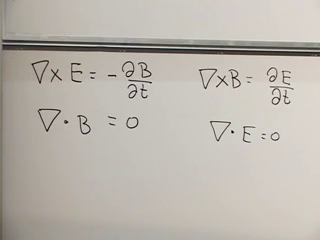
\includegraphics[width=0.76\textwidth]{lecture_58_figure_06.png}
\caption{四つの真空マクスウェル方程式。電場と磁場のほぼ対称性を示すように配置されている。}
\lectureframe{00:27:30}
\end{figure}

電荷密度\(\rho\)は最終的に式~\eqref{eq:gauss-e-vac}の右辺のゼロを置き換え、電流密度\(\mathbf J\)は式~\eqref{eq:ampere-vac}に入る。これらの項は一時的に延期する。源のない方程式は、変換構造と波動の仕組みを最も少ない雑多な要素で明らかにする。

それらはまたアインシュタインの難問を際立たせる。波を追いかけるガリレイ的観測者は、速度を差し引いてより小さな波の速さを測ることを期待するであろう。しかし、同じマクスウェル方程式がすべての慣性系で成り立つなら、各観測者は同じ単位波の速さを導く。打開策は、枠ごとに波動方程式を変えることではない。ローレンツ変換を用い、変換則がすでに知られている対象の中にマクスウェル方程式を示すことである。

\section{電場と磁場を一つのテンソルとして}

電場と磁場は反対称場テンソル
\begin{equation}
F^{\mu\nu}=
\begin{pmatrix}
0   & -E_x & -E_y & -E_z\\
E_x & 0    & -B_z & B_y\\
E_y & B_z  & 0    & -B_x\\
E_z & -B_y & B_x  & 0
\end{pmatrix},
\label{eq:l0203-field-tensor}
\end{equation}
に結合する。ここで行と列の順序は\(t,x,y,z\)である。反対称性
\begin{equation}
F^{\mu\nu}=-F^{\nu\mu},
\end{equation}
は対角成分をゼロにし、行列の下半分を上半分から決定する。時間-空間成分は\(\mathbf E\)を含み、純粋に空間的な成分は\(\mathbf B\)を含む。

\begin{figure}[H]
\centering
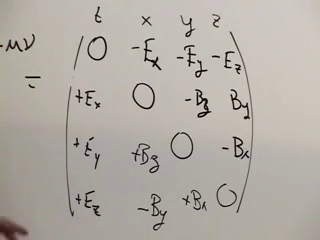
\includegraphics[width=0.58\textwidth]{lecture_58_figure_03.png}
\caption{完成した電磁場テンソル。その電場成分と磁場成分を含む。}
\lectureframe{00:32:05}
\end{figure}

\(F^{\mu\nu}\)の重要性は、六つの場の成分が一つの行列に収まることだけではない。ローレンツ変換の下で、それは二階のテンソルとして変換する。したがって、異なる観測者が測定する電場と磁場は、対象全体が整合的に変換するために必要な仕方で正確に混ざり合う。

第二の反対称テンソル、双対場テンソル\(\widetilde F^{\mu\nu}\)がある。現在の規約では、それは式~\eqref{eq:l0203-field-tensor}から置き換え
\begin{equation}
\mathbf E\longmapsto-\mathbf B,
\qquad
\mathbf B\longmapsto\mathbf E.
\label{eq:dual-replacement}
\end{equation}
によって得られる。したがって
\begin{equation}
\widetilde F^{\mu\nu}=
\begin{pmatrix}
0    & B_x  & B_y  & B_z\\
-B_x & 0    & -E_z & E_y\\
-B_y & E_z  & 0    & -E_x\\
-B_z & -E_y & E_x  & 0
\end{pmatrix}.
\label{eq:dual-tensor}
\end{equation}
である。式~\eqref{eq:dual-replacement}の符号は重要である。講義はまず電場と磁場の交換を言葉で試み、符号の不一致に気づき、行列を完成させる前にそれを訂正する。

\begin{figure}[H]
\centering
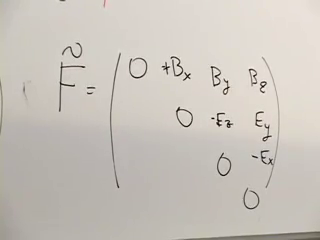
\includegraphics[width=0.58\textwidth]{lecture_58_figure_07.png}
\caption{必要な符号とともに電場と磁場の成分を交換して組み立てられる双対テンソル。}
\lectureframe{00:35:45}
\end{figure}

\section{共変形の真空方程式}

各マクスウェル方程式は1つの微分を含む。2階のテンソルから出発し、1つの微分添字を縮約すると1つの自由添字が残るので、自然な共変的候補は
\begin{align}
\partial_\mu F^{\mu\nu}&=0,
\label{eq:maxwell-covariant-vac}\\
\partial_\mu\widetilde F^{\mu\nu}&=0.
\label{eq:maxwell-dual-vac}
\end{align}
である。\(\nu\)の各固定値に対して、式~\eqref{eq:maxwell-covariant-vac}は1つの方程式である。\(\nu\)は\(t,x,y,z\)であり得るので、これは4つのスカラー方程式をまとめたものである。式~\eqref{eq:maxwell-dual-vac}は残りの4つをまとめたものである。これは元のリストにおける2つのベクトル回転方程式と2つのスカラー発散方程式に対応する。

簡潔な記法は、それがよく知られた方程式を再現する場合にのみ有用である。\(\nu=z\)とすると、
\begin{align}
\partial_\mu F^{\mu z}
&=\partial_tF^{tz}
  +\partial_xF^{xz}
  +\partial_yF^{yz}
  +\partial_zF^{zz}\\
&=-\partial_tE_z+\partial_xB_y-\partial_yB_x\\
&=-\partial_tE_z+
  \bigl(\boldsymbol\nabla\times\mathbf B\bigr)_z.
\end{align}
項\(F^{zz}\)は反対称性により消える。結果をゼロと置くと、
\begin{equation}
\boldsymbol\nabla\times\mathbf B=\partial_t\mathbf E.
\end{equation}
の\(z\)成分が得られる。\(x\)成分と\(y\)成分は添字を巡回させることで従う。

\begin{figure}[H]
\centering
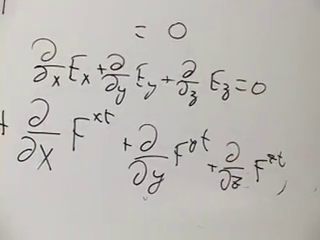
\includegraphics[width=0.76\textwidth]{lecture_58_figure_08.png}
\caption{共変場の方程式の成分展開。対角テンソル成分は消え、残りの項がマクスウェル方程式を再構成する。}
\lectureframe{00:43:30}
\end{figure}

次に時間成分を取る：
\begin{align}
\partial_\mu F^{\mu t}
&=\partial_tF^{tt}
  +\partial_xF^{xt}
  +\partial_yF^{yt}
  +\partial_zF^{zt}\\
&=\partial_xE_x+\partial_yE_y+\partial_zE_z\\
&=\boldsymbol\nabla\cdot\mathbf E.
\end{align}
したがってこれは式~\eqref{eq:gauss-e-vac}を与える。双対テンソルについて同じ検査を行うと、
\(\boldsymbol\nabla\cdot\mathbf B=0\) および
\(\boldsymbol\nabla\times\mathbf E=-\partial_t\mathbf B\) が得られる。

簡潔な方程式は今や単に推測されたのではなく確立された。それらの自由添字構造はそれらを4元ベクトル方程式にするので、ローレンツ変換はそれらの成分を変えるが形は変えない。これが、真空マクスウェル方程式がすべての慣性系で同じであるという正確な意味である。

\section{一次方程式から波動へ}

マクスウェル方程式は1階微分のみを含むのに対し、波動方程式は2階微分を含む。この見かけの不一致は、マクスウェルの理論が2つの場を結合するために解消される。\(\mathbf E\)と\(\mathbf B\)に対する1階方程式の対は、どちらか一方の場だけに対する2階方程式に組み合わせることができる。

式~\eqref{eq:ampere-vac}を時間で微分する：
\begin{equation}
\partial_t^2\mathbf E
=\boldsymbol\nabla\times\partial_t\mathbf B.
\end{equation}
ファラデーの法則が\(\mathbf B\)の時間微分を与え、
\begin{equation}
\partial_t\mathbf B=-\boldsymbol\nabla\times\mathbf E,
\end{equation}
したがって
\begin{equation}
\partial_t^2\mathbf E
=-\boldsymbol\nabla\times
  \bigl(\boldsymbol\nabla\times\mathbf E\bigr).
\label{eq:double-curl}
\end{equation}

黒板では記憶した恒等式を呼び出すのではなく、1つの成分を計算する。\(x\)成分について、
\begin{align}
\bigl[\boldsymbol\nabla\times
(\boldsymbol\nabla\times\mathbf E)\bigr]_x
&=\partial_y(\boldsymbol\nabla\times\mathbf E)_z
 -\partial_z(\boldsymbol\nabla\times\mathbf E)_y\\
&=\partial_y(\partial_xE_y-\partial_yE_x)\\
&\quad-\partial_z(\partial_zE_x-\partial_xE_z)\\
&=\partial_x(\partial_yE_y+\partial_zE_z)
 -\partial_y^2E_x\\
&\quad-\partial_z^2E_x.
\end{align}
\(\partial_x^2E_x\)を加えて引くことで発散をあらわにする：
\begin{align}
\bigl[\boldsymbol\nabla\times
(\boldsymbol\nabla\times\mathbf E)\bigr]_x
&=\partial_x(\boldsymbol\nabla\cdot\mathbf E)
 -\nabla^2E_x.
\label{eq:double-curl-x}
\end{align}
真空中では\(\boldsymbol\nabla\cdot\mathbf E=0\)。式~\eqref{eq:double-curl}と\eqref{eq:double-curl-x}を組み合わせると
\begin{equation}
\left(\partial_t^2-\nabla^2\right)E_x=0.
\label{eq:ex-wave}
\end{equation}

\begin{figure}[H]
\centering
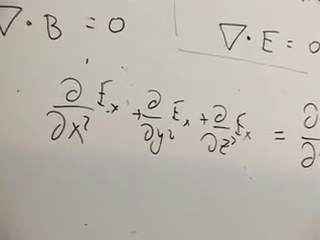
\includegraphics[width=0.72\textwidth]{lecture_58_figure_09.png}
\caption{成分計算により\(E_x\)に対する波動方程式に到達する。}
\lectureframe{00:57:10}
\end{figure}

同じ計算が\(E_y\)と\(E_z\)にも適用され、同様の消去により
\begin{equation}
\left(\partial_t^2-\nabla^2\right)\mathbf B=0.
\end{equation}
が得られる。したがって電場と磁場は真空中を波として伝播することができる。ここで用いた単位ではそれらの速さは1であり、これは通常の単位に戻すと速さが\(c\)であることを意味する。

\section{平面波とその偏光}

正の\(z\)方向に進む単純な波を構成する：
\begin{equation}
\mathbf E(z,t)
=\widehat{\mathbf x}\,E_0
  \cos\!\bigl(k(z-t)\bigr).
\label{eq:plane-e}
\end{equation}
そのプロファイルは形を変えずに\(z\)に沿って平行移動する。電場が\(x\)軸に沿って向くので、波は\(x\)方向に直線偏光している。例を単純に保つために\(E_y=0\)を選んだだけであり、第2の横偏光を含めることもできた。

縦成分は同じようには自由ではない。波は\(z\)と\(t\)のみに依存するので、
\begin{equation}
\boldsymbol\nabla\cdot\mathbf E
=\partial_zE_z=0.
\end{equation}
したがって\(E_z\)は定数であり得るが、変動する波のプロファイルを含むことはできない。一様な背景場は独立に重ね合わせたり取り除いたりできる；それは伝播する放射の一部ではない。波自体は横波である：
\begin{equation}
\mathbf E_{\mathrm{wave}}\cdot\widehat{\mathbf z}=0.
\end{equation}

ファラデーの法則が磁場を定める。式~\eqref{eq:plane-e}に対して、\(\boldsymbol\nabla\times\mathbf E\)の唯一の非零成分は\(y\)成分であり、
\begin{equation}
(\boldsymbol\nabla\times\mathbf E)_y=\partial_zE_x.
\end{equation}
したがって\(\partial_t\mathbf B\)は\(y\)に沿って向き、整合する選択は
\begin{equation}
\mathbf B(z,t)
=\widehat{\mathbf y}\,E_0
  \cos\!\bigl(k(z-t)\bigr).
\label{eq:plane-b}
\end{equation}
である。これらの単位では電場と磁場の振幅は等しい。それらの向きは
\begin{equation}
\mathbf E\perp\mathbf B,
\qquad
\mathbf E\perp\widehat{\mathbf z},
\qquad
\mathbf B\perp\widehat{\mathbf z},
\qquad
\mathbf E\times\mathbf B\parallel\widehat{\mathbf z}.
\end{equation}
に従う。

\begin{figure}[H]
\centering
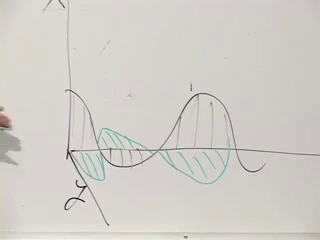
\includegraphics[width=0.70\textwidth]{lecture_58_figure_05.png}
\caption{横電磁波の完成した黒板スケッチ：電場と磁場の振動は互いに垂直であり、伝播方向にも垂直である。}
\lectureframe{01:05:25}
\end{figure}

\begin{figure}[H]
\centering
\scalebox{0.90}{%
\begin{tikzpicture}[x=1cm,y=1cm,>=Latex]
  \draw[->,thick] (0,0) -- (8.2,0) node[right] {$z$};
  \draw[->,thick] (0,-1.6) -- (0,1.7) node[above] {$x$};
  \draw[->,thick] (0,0) -- (-1.15,-0.8) node[below left] {$y$};
  \draw[blue!70!black,thick,domain=0:7.5,samples=120]
    plot (\x,{0.95*sin(90*\x)});
  \foreach \z/\s in {0.8/1,2.8/-1,4.8/1,6.8/-1}{
    \draw[->,green!45!black,thick]
      (\z,0) -- ++({-0.55*\s},{-0.38*\s});
  }
  \node[blue!70!black] at (6.9,1.25) {$\mathbf E$};
  \node[green!45!black] at (5.2,-1.05) {$\mathbf B$};
  \draw[->,very thick] (6.2,1.55) -- (7.7,1.55)
    node[midway,above] {propagation};
\end{tikzpicture}
}
\caption{場\(\mathbf E\)と\(\mathbf B\)は互いに垂直であり、伝播方向にも垂直である。}
\end{figure}

これが光および真空中のすべての電磁放射の特徴である。波を生み出した方程式がローレンツ共変であるので、別の慣性観測者もまた、\(c\)で進み、横方向の電場と磁場をもつ電磁波を記述する。

\section{電荷密度と電流密度}

ここで、一時的に脇に置いていた源を復元する。多数の荷電粒子が領域を占めるとき、それらを連続的な電荷密度に粗視化すると便利である。
\begin{equation}
\rho(\mathbf x,t)=\frac{dQ}{dV}.
\end{equation}
この近似は、水が分子から成るにもかかわらず連続的な流体として扱うことに似ている。正電荷と負電荷は逆の符号で寄与するので、\(\rho\) は単位体積あたりの正味の電荷である。

選んだ領域 \(V\) 内の電荷は
\begin{equation}
Q_V(t)=\int_V\rho(\mathbf x,t)\,dV.
\label{eq:charge-volume}
\end{equation}
である。密度は位置と時間によって変化しうる。電荷の山はある点から離れて移動し、そこでの局所的な密度を変化させうる。しかし、それが任意の仕方で変化することはできない。自然は電荷を保存する。

大域的な保存だけでは弱すぎる。それは、全電荷が変わらないまま、電荷が地球から消えて同時に火星に現れることを許してしまう。より強い主張は局所的なものである。電荷は、一つの場所を離れて別の場所に到達するには、その間の空間における流れを通じてのみ可能である。

その流れを記述するために、無限小の向き付けられた面要素
\begin{equation}
d\boldsymbol\sigma=\widehat{\mathbf n}\,d\sigma.
\end{equation}
を取る。その大きさは面積であり、その向きは面に垂直である。電流密度 \(\mathbf J\) は、単位時間あたりにその要素を横切る電荷が
\begin{equation}
\frac{dQ}{dt}=\mathbf J\cdot d\boldsymbol\sigma.
\label{eq:current-flux-element}
\end{equation}
となるように定義される。\(\mathbf J\) の大きさは単位面積・単位時間あたりの電荷であり、その向きは正電荷の流れの向きである。

\begin{figure}[H]
\centering
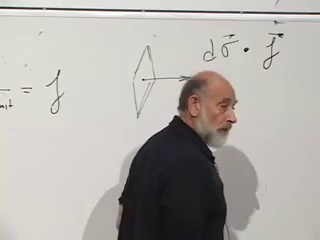
\includegraphics[width=0.64\textwidth]{lecture_58_figure_10.png}
\caption{向き付けられた面積要素とフラックス因子 \(d\boldsymbol\sigma\cdot\mathbf J\)。}
\lectureframe{01:18:15}
\end{figure}

内積は面に垂直な成分を選び出す。面に接する電流はどちらの側も横切らず、寄与はゼロである。法線に平行な電流は、大きさを固定すれば最大のフラックスを与える。導線の電流は一つの特別な場合であるが、\(\mathbf J\) はシートを通って流れる電荷や三次元空間全体を流れる電荷も記述しうる。

\section{局所保存と連続の方程式}

空間内の領域 \(V\) を固定し、その閉境界 \(\partial V\) のすべての要素を外向きに配向する。正味の外向き電流があれば、内部の電荷は減少する：
\begin{equation}
\frac{dQ_V}{dt}
=-\oint_{\partial V}\mathbf J\cdot d\boldsymbol\sigma.
\label{eq:integral-conservation}
\end{equation}
負号は慣習ではなく物理的である。正の外向きフラックスは領域から正電荷を取り除く。式~\eqref{eq:charge-volume} を用いると、
\begin{equation}
\int_V\partial_t\rho\,dV
=-\oint_{\partial V}\mathbf J\cdot d\boldsymbol\sigma.
\label{eq:integral-continuity-one}
\end{equation}

\begin{figure}[H]
\centering
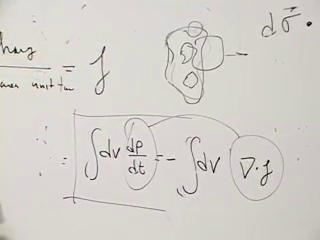
\includegraphics[width=0.72\textwidth]{lecture_58_figure_11.png}
\caption{表面フラックスを体積に関する表現に変換した後の固定領域の保存則。}
\lectureframe{01:29:00}
\end{figure}

ガウスの定理は、発散定理とも呼ばれ、閉曲面を通るフラックスとその内部の発散を関係づける：
\begin{equation}
\oint_{\partial V}\mathbf A\cdot d\boldsymbol\sigma
=\int_V\boldsymbol\nabla\cdot\mathbf A\,dV.
\label{eq:divergence-theorem}
\end{equation}
容器の内部の点で水を注入する隠れたパイプを思い描くことができる。発散は、パイプの端から水が現れる局所的な割合を測り、面積分は容器を出る水の総量を測る。内部で外向きの流れとして生成されるものは、最終的に境界を横切らなければならない。

式~\eqref{eq:divergence-theorem} を \(\mathbf J\) に適用すると
\begin{equation}
\int_V
\left(\partial_t\rho+\boldsymbol\nabla\cdot\mathbf J\right)dV=0.
\end{equation}
が得られる。この関係はあらゆる可能な領域 \(V\) に対して成り立つ。したがって被積分関数は点ごとに消えなければならない：
\begin{equation}
\boxed{\partial_t\rho+\boldsymbol\nabla\cdot\mathbf J=0.}
\label{eq:continuity-three}
\end{equation}

\begin{figure}[H]
\centering
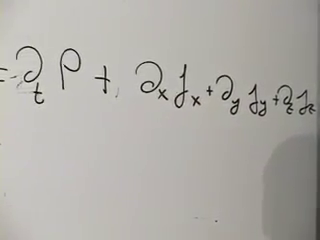
\includegraphics[width=0.72\textwidth]{lecture_58_figure_12.png}
\caption{成分ごとに書いた局所的な連続の方程式。}
\lectureframe{01:29:50}
\end{figure}

式~\eqref{eq:continuity-three} は、局所保存が要求することを正確に述べている。ある点または小さな領域内で電荷密度が減少するならば、電流はそこから外向きに発散しなければならない。電流が内向きに収束するならば、電荷密度は増加する。

密度と電流は自然に四元電流
\begin{equation}
J^\mu=(\rho,J_x,J_y,J_z)
\label{eq:four-current}
\end{equation}
を \(c=1\) 単位で形成する。連続の方程式はローレンツスカラー方程式
\begin{equation}
\partial_\mu J^\mu=0.
\label{eq:continuity-four}
\end{equation}
となる。相対論的な分布の流れは、一つの粒子の四元速度がそうであるように、四元ベクトルとして変換されるべきである。式~\eqref{eq:continuity-four} は、局所的な電荷保存をすべての慣性系で有効にする。

\section{源を含むマクスウェル方程式}

電荷と電流を復元すると
\begin{align}
\boldsymbol\nabla\cdot\mathbf E&=\rho,
\label{eq:gauss-e-source}\\
\boldsymbol\nabla\cdot\mathbf B&=0,\\
\boldsymbol\nabla\times\mathbf E&=-\partial_t\mathbf B,\\
\boldsymbol\nabla\times\mathbf B&=\partial_t\mathbf E+\mathbf J.
\label{eq:ampere-source}
\end{align}
が得られる。電気的な源を含む方程式は
\begin{equation}
\boxed{\partial_\mu F^{\mu\nu}=J^\nu,}
\label{eq:maxwell-source-covariant}
\end{equation}
にまとまり、源のない磁気的な対は
\begin{equation}
\boxed{\partial_\mu\widetilde F^{\mu\nu}=0.}
\label{eq:maxwell-dual-source}
\end{equation}
のままである。

\begin{figure}[H]
\centering
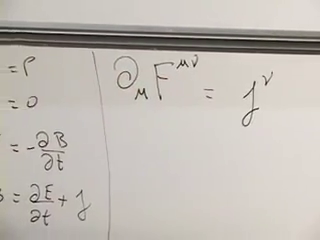
\includegraphics[width=0.78\textwidth]{lecture_58_figure_13.png}
\caption{源を含むマクスウェル方程式とその共変形 \(\partial_\mu F^{\mu\nu}=J^\nu\)。}
\lectureframe{01:34:00}
\end{figure}

式~\eqref{eq:maxwell-source-covariant} の時間成分は
\begin{equation}
\partial_\mu F^{\mu t}=J^t=\rho,
\end{equation}
と読め、すでに行った成分計算によりその左辺は
\(\boldsymbol\nabla\cdot\mathbf E\) となる。三つの空間成分は
\(\boldsymbol\nabla\times\mathbf B=\partial_t\mathbf E+\mathbf J\)
を再現する。

有用な整合性の検査もある。\(\partial_\nu\) を
式~\eqref{eq:maxwell-source-covariant} に適用すると
\begin{equation}
\partial_\nu J^\nu
=\partial_\nu\partial_\mu F^{\mu\nu}=0,
\end{equation}
が得られる。なぜなら二つの導関数は \(\mu\leftrightarrow\nu\) の下で対称であるのに対し、\(F^{\mu\nu}\) は反対称だからである。\editorialnote{この短い整合性の検査は共変方程式から従い、マクスウェル方程式が源を含む形で連続の方程式を自動的に尊重する理由を明示する。}

相反構造はこれで完成した。テンソル的な力の法則
\(f^\mu=qF^\mu{}_\nu u^\nu\) は場が電荷にどのように作用するかを記述し、
式~\eqref{eq:maxwell-source-covariant} は電荷と電流が場をどのように生成するかを記述する。両者はテンソル方程式である。真空中では、同じ場の方程式から \(c\) で進む横波が得られる。したがって、ローレンツ共変性と電磁波方程式は、この構成の動機となった点で一致する。すなわち、すべての慣性観測者が同じ電磁気学の法則と同じ光速度を得るのである。